\chapter{\textit{User Research}}
\label{ch:user_research}

\begin{chapterabstract}
Investigación mixta para precisar el problema de ImprontIA: una \textbf{encuesta a 213 estudiantes} ($N=213$) de UADE, UBA y Universidad Siglo 21, y \textbf{tres entrevistas semiestructuradas} a responsables de educación a distancia, docencia e investigación. La transparencia previa y la revisión humana resultaron las condiciones más valoradas (\textbf{93,0\,\%} y \textbf{93,9\,\%} respectivamente), mientras que la ausencia de cámara no se asoció necesariamente con menor invasividad percibida. Los hallazgos triangulados orientan directamente los Requerimientos (Capítulo~\ref{ch:requerimientos}) y el análisis de Competencias (Sección~\ref{ch:competencias}).
\end{chapterabstract}

\section{Objetivo y alcance}

El \textit{User Research} se realizó con el propósito de profundizar la comprensión del problema abordado por ImprontIA a partir de evidencia obtenida de personas vinculadas con las evaluaciones digitales. En particular, se buscó relevar percepciones, experiencias y dificultades asociadas con estas instancias de evaluación, así como las condiciones bajo las cuales se desarrollan, supervisan y revisan. El estudio permitió incorporar al análisis la perspectiva de estudiantes y de actores con experiencia docente y de gestión académica, complementando la caracterización conceptual y técnica desarrollada en los capítulos anteriores.

El alcance de esta etapa se concentró en comprender y precisar el problema, sin utilizar el \textit{User Research} como mecanismo de validación directa de ImprontIA. Por lo tanto, la investigación no se orientó a determinar si los participantes utilizarían la plataforma ni a medir intención de uso o aceptación de una solución previamente definida. Cuando durante las entrevistas se presentaron características de la propuesta y se solicitaron opiniones sobre ellas, esos segmentos fueron tratados de manera diferenciada respecto de la exploración previa del problema.

\section{Metodología}

El \textit{User Research} se desarrolló mediante un enfoque mixto, combinando una encuesta dirigida a estudiantes con entrevistas semiestructuradas a perfiles vinculados con la docencia, la investigación y la gestión académica. Ambas técnicas se utilizaron de manera complementaria: la encuesta permitió relevar de forma estructurada percepciones y experiencias dentro de una muestra más amplia de estudiantes, mientras que las entrevistas permitieron profundizar en el contexto de las evaluaciones, los criterios que intervienen en su diseño y revisión y las condiciones institucionales y operativas asociadas a estas instancias.

La encuesta se difundió a través de WhatsApp, grupos vinculados con facultades y universidades, y compañeros y contactos estudiantiles. La difusión alcanzó estudiantes de distintas instituciones, entre ellas UADE, UBA y Universidad Siglo 21. Al comienzo del formulario se informó que la encuesta formaba parte de un trabajo universitario, que la participación era voluntaria y que las respuestas eran anónimas. De acuerdo con el procedimiento de reclutamiento utilizado, se trabajó con una muestra no probabilística por conveniencia.

El formulario original recibió 218 respuestas correspondientes a diferentes perfiles. Para el análisis cuantitativo se decidió trabajar exclusivamente con estudiantes universitarios o terciarios, por lo que se excluyeron cinco respuestas pertenecientes a perfiles no estudiantiles. De este modo, se analizaron 213 respuestas de estudiantes ($N=213$). El análisis cuantitativo fue de carácter descriptivo y se orientó a examinar las distribuciones correspondientes a las variables definidas en el instrumento (Apéndice~\ref{apx:encuesta}). En consecuencia, los resultados describen las percepciones de la muestra relevada y no se consideran generalizables a la totalidad de la población universitaria. Dentro de la muestra se observó un predominio de participantes pertenecientes a Ingeniería, Tecnología e Informática.

Para el componente cualitativo se seleccionaron de manera intencional participantes con distintos perfiles académicos y profesionales que pudieran aportar perspectivas relevantes sobre evaluaciones digitales, docencia y gestión académica. Se realizaron tres entrevistas virtuales semiestructuradas, que se identifican con un código y el perfil de cada participante (Tabla~\ref{tab:ur_entrevistas}).

\begin{table}[htbp]
    \caption{Participantes de las entrevistas}
    \label{tab:ur_entrevistas}
    \centering
    \small
    \begin{tabularx}{\textwidth}{l >{\raggedright\arraybackslash}X l}
        \toprule
        \tblhead \textbf{Código} & \textbf{Perfil} & \textbf{Fecha} \\
        \midrule
        ENT-01 & Gestión académica de la educación en línea (responsable del área en una universidad privada) & 9/6/2026 \\
        ENT-02 & Docente universitario e investigador en ciencias biomédicas & 10/6/2026 \\
        ENT-03 & Gestión de la educación a distancia en facultades de ingeniería y ciencias económicas & 10/6/2026 \\
        \bottomrule
    \end{tabularx}
\end{table}

Las transcripciones completas se reproducen en el Apéndice~\ref{apx:entrevistas}. Dos de los entrevistados (ENT-01 y ENT-03) trabajan en UADE Online, el área de educación a distancia de la universidad de los autores; este vínculo se declara como posible sesgo en la Sección~\ref{sec:ur_limitaciones}.

Antes de realizar las entrevistas se informó a los participantes que la conversación formaba parte del Proyecto Final, que sería grabada y posteriormente transcripta, y se solicitó autorización para utilizar su nombre e identificación profesional en el trabajo. Los tres participantes autorizaron estas condiciones. Aun con esa autorización, en el análisis se los identifica por código y perfil, como es habitual en la investigación cualitativa, para que la atención recaiga en los argumentos y no en las personas; su identificación completa (nombre, título y rol) figura solo en la ficha de cada entrevista del Apéndice~\ref{apx:entrevistas}. No se consignan matrículas ni registros profesionales porque no corresponden a las funciones docentes, de investigación y de gestión académica relevadas. Las entrevistas se realizaron utilizando una guía orientativa de preguntas que no funcionó como un cuestionario rígido: durante las conversaciones se modificó el orden de los temas cuando resultó necesario, se profundizaron aspectos relevantes y se realizaron repreguntas de acuerdo con el desarrollo de cada entrevista. Posteriormente, las conversaciones se transcribieron y las transcripciones se analizaron mediante un proceso de codificación temática (Apéndice~\ref{apx:cualitativo}), utilizado para organizar los contenidos relevantes en torno a temas comunes y conservar, al mismo tiempo, las diferencias de contexto y perspectiva entre los participantes.

Para reducir el riesgo de interpretar como hallazgos espontáneos opiniones condicionadas por la presentación de la propuesta, las entrevistas se organizaron diferenciando una etapa de exploración (\textit{discovery}) de una instancia de retroalimentación posterior (\textit{feedback}). En las entrevistas ENT-01 y ENT-02, la exploración inicial del problema se llevó a cabo antes de presentar ImprontIA. En ENT-03, en cambio, se presentó una descripción general del proyecto al comienzo de la conversación, por lo que sus aportes fueron analizados teniendo en cuenta esta diferencia metodológica y no se consideraron directamente equivalentes a los obtenidos en la etapa de exploración de las otras entrevistas. Además, los entrevistadores tenían con ENT-02 un vínculo previo docente--alumno de la carrera, que puede haber favorecido respuestas más cercanas o complacientes; ese vínculo se considera un posible sesgo y se tuvo en cuenta al ponderar sus aportes, que se contrastaron con los de las otras dos entrevistas y con la encuesta.

Finalmente, se integraron los resultados obtenidos mediante ambas técnicas a través de una instancia de triangulación (Apéndice~\ref{apx:triangulacion}). Este proceso mantuvo diferenciada la naturaleza de cada fuente y permitió organizar relaciones de convergencia, complementariedad y evidencia aportada por una única técnica, sin tratar la encuesta y las entrevistas como mediciones equivalentes del mismo fenómeno.

\section{Resultados de la encuesta a estudiantes}

Los resultados de la encuesta permiten caracterizar distintas dimensiones de la experiencia y percepción estudiantil frente a las evaluaciones digitales. Para el cuerpo principal se seleccionaron aquellos resultados que aportan de forma más directa a la comprensión del problema: la confiabilidad atribuida a estas instancias, los riesgos asociados con su integridad, la percepción de distintos mecanismos de supervisión y las condiciones consideradas relevantes para que su aplicación resulte académicamente defendible. Los resultados corresponden a la muestra relevada de 213 estudiantes y deben interpretarse dentro de ese alcance.

\begin{figure}[h!]
    \centering
    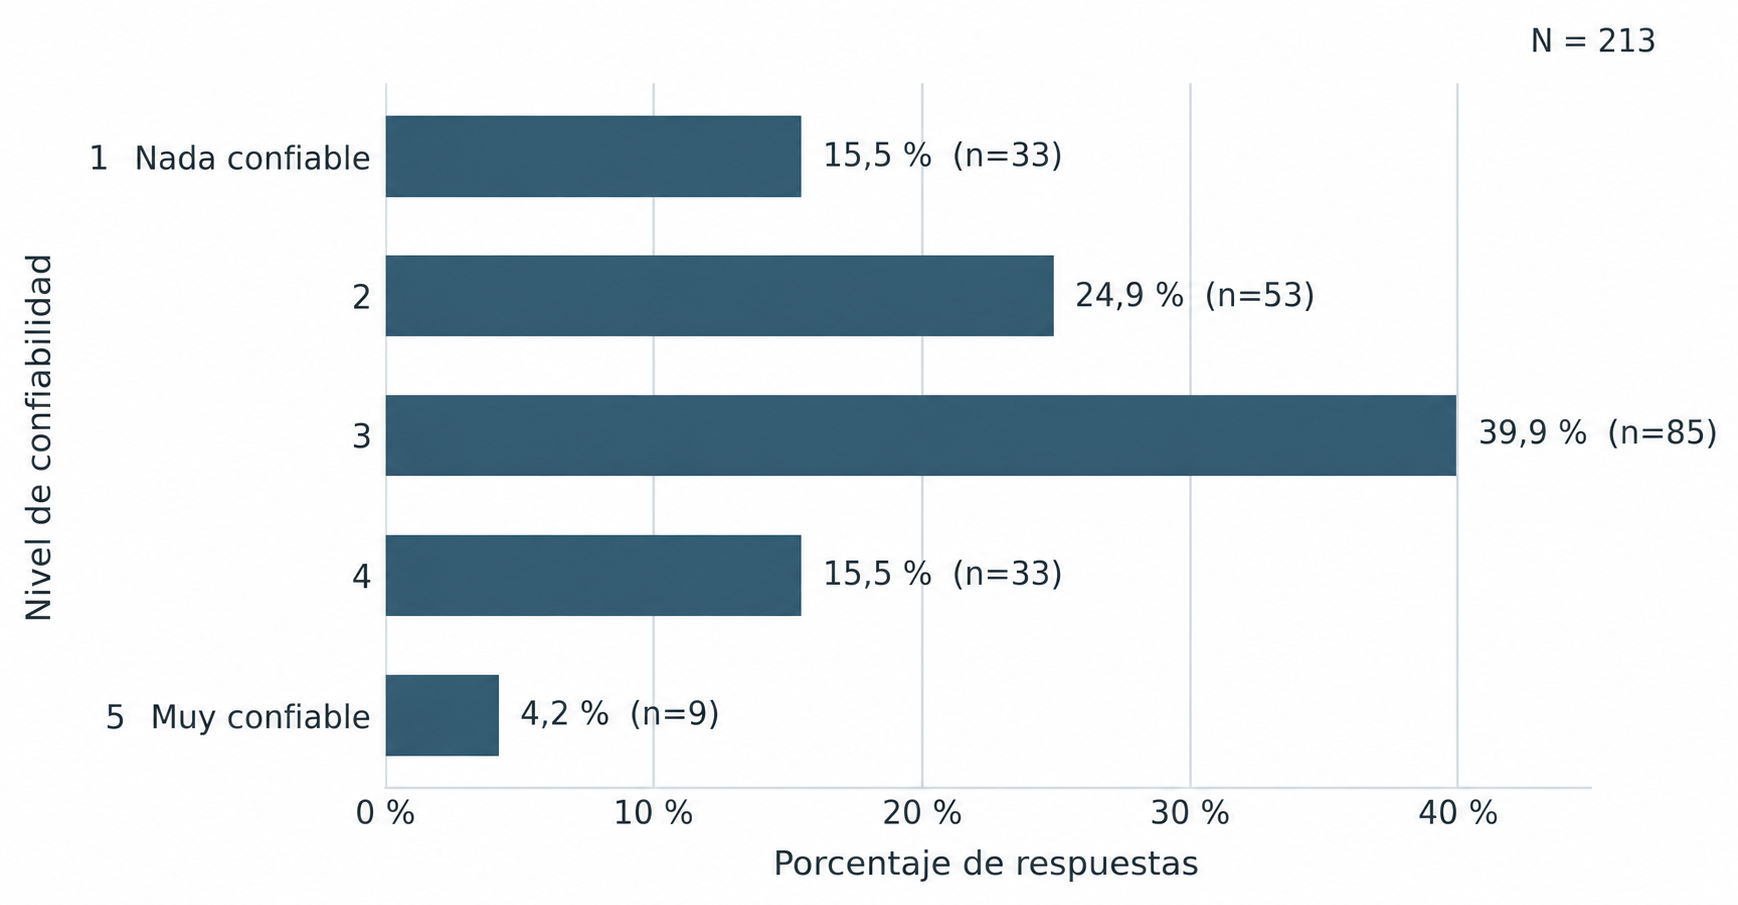
\includegraphics[width=0.85\textwidth]{./figures/ur_fig1_confiabilidad}
    \caption[Confiabilidad percibida de las evaluaciones digitales]{Confiabilidad percibida de las evaluaciones digitales. Fuente: elaboración propia a partir de la encuesta de \textit{User Research}, $N=213$.}
    \label{fig:ur_confiabilidad}
\end{figure}

La confiabilidad percibida se concentró principalmente en niveles bajos e intermedios. En la pregunta sobre confiabilidad de las evaluaciones digitales (EST05), el \textbf{40,4\,\%} de la muestra se ubicó en los valores 1--2 de la escala y otro \textbf{39,9\,\%} seleccionó el punto medio, mientras que el \textbf{19,7\,\%} manifestó niveles altos de confiabilidad. La distribución no permite afirmar que exista un rechazo generalizado hacia las evaluaciones digitales, pero sí muestra que la confianza elevada constituye una posición minoritaria dentro de la muestra.

\begin{figure}[h!]
    \centering
    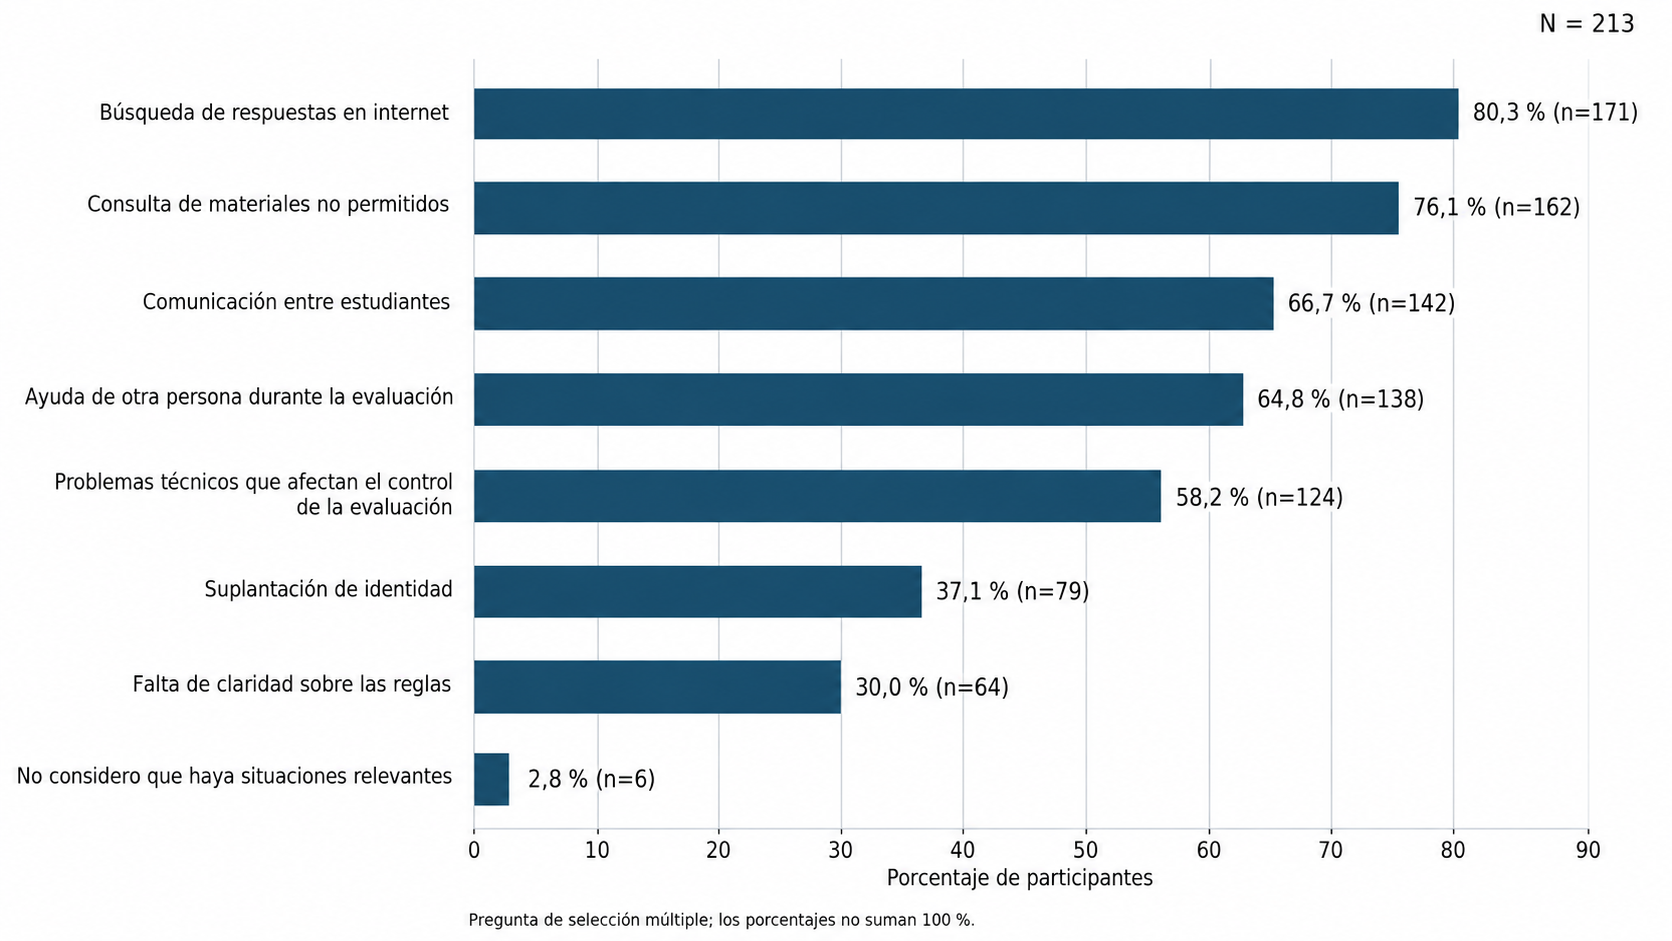
\includegraphics[width=0.85\textwidth]{./figures/ur_fig2_riesgos}
    \caption[Situaciones percibidas como riesgos para la integridad de una evaluación digital]{Situaciones percibidas como riesgos para la integridad de una evaluación digital (pregunta de selección múltiple; los porcentajes no suman 100\,\%). Fuente: elaboración propia a partir de la encuesta de \textit{User Research}, $N=213$.}
    \label{fig:ur_riesgos}
\end{figure}

Las respuestas a la pregunta sobre situaciones percibidas como riesgos para la integridad (EST07) muestran que la integridad de una evaluación digital no es percibida como un problema asociado a una única conducta. Entre las situaciones más seleccionadas aparecen la búsqueda de respuestas en internet, la consulta de materiales no permitidos, la comunicación entre estudiantes y la ayuda de terceros. También se señalaron problemas técnicos capaces de afectar las condiciones de control. Dado que se trató de una pregunta de selección múltiple, estos resultados expresan qué situaciones fueron reconocidas como riesgos por los participantes y no la frecuencia real con que dichas conductas ocurren durante una evaluación.

En conjunto, el resultado permite caracterizar el problema como multidimensional: diferentes formas de asistencia externa, interacción entre personas y condiciones técnicas pueden afectar el proceso evaluativo. Por esta razón, los datos no sostienen una interpretación de la integridad basada exclusivamente en una única señal o modalidad de comportamiento.

\begin{figure}[h!]
    \centering
    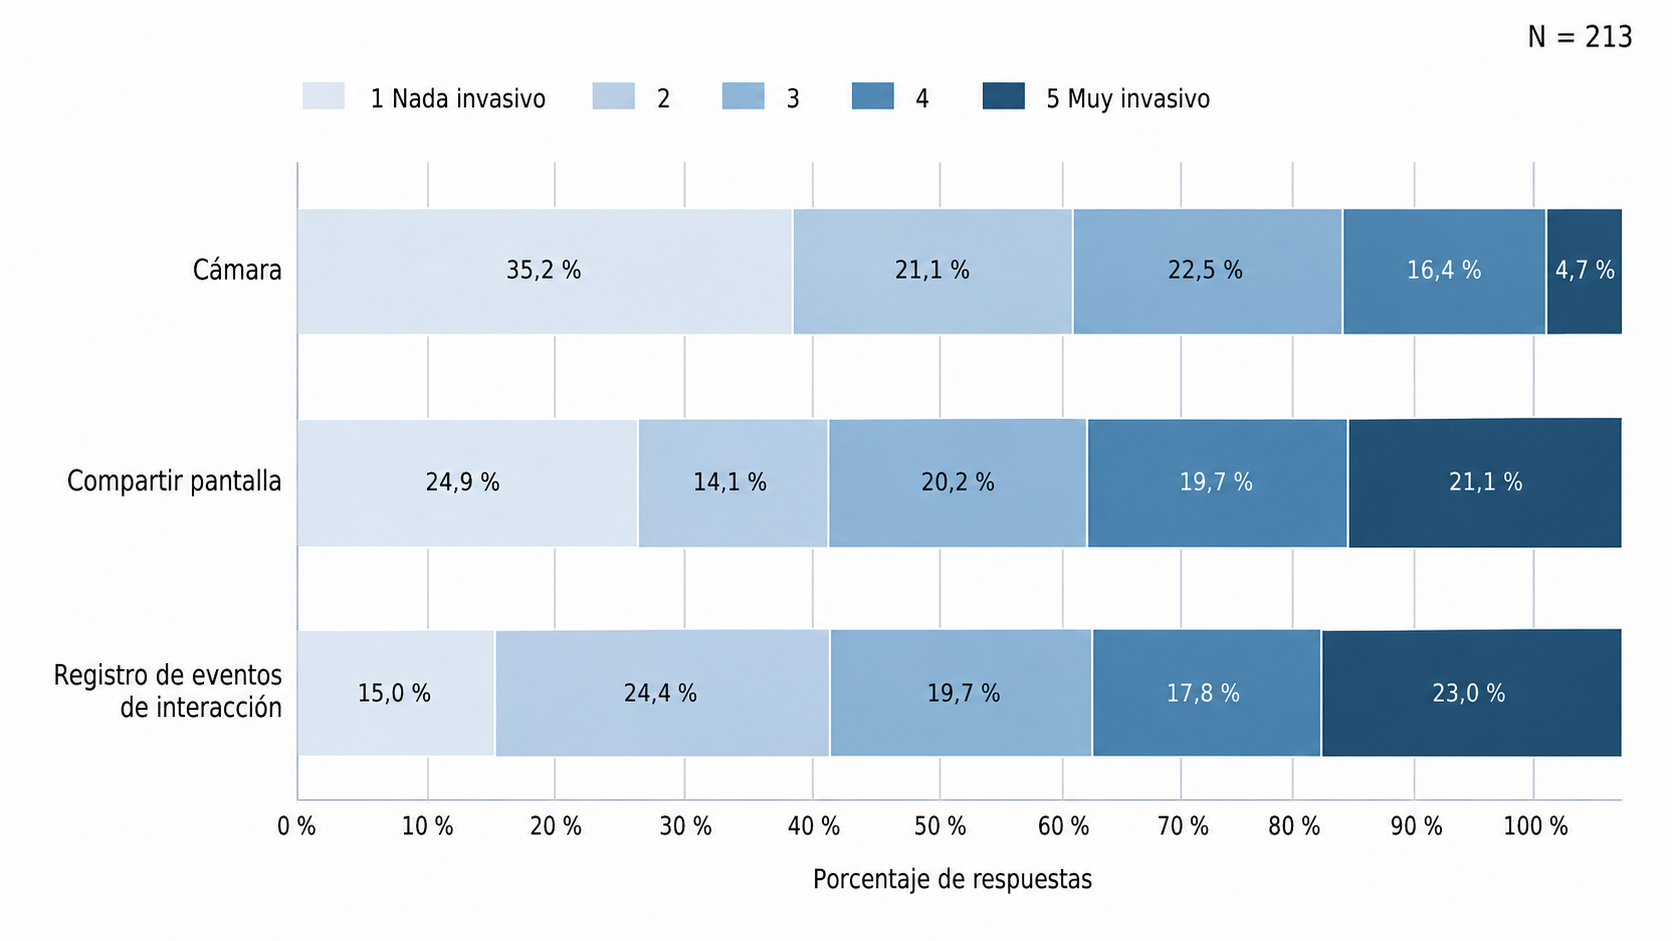
\includegraphics[width=0.85\textwidth]{./figures/ur_fig3_invasividad}
    \caption[Percepción de invasividad según el mecanismo de supervisión]{Percepción de invasividad según el mecanismo de supervisión. Fuente: elaboración propia a partir de la encuesta de \textit{User Research}, $N=213$.}
    \label{fig:ur_invasividad}
\end{figure}

La percepción de invasividad varió según el mecanismo presentado y no mostró una jerarquía simple entre las alternativas. La cámara concentró una mayor proporción de valoraciones en los niveles bajos de invasividad, mientras que compartir pantalla y registrar eventos de interacción produjeron distribuciones más divididas. En particular, el registro de eventos no fue percibido de manera homogénea como una alternativa menos invasiva.

Este resultado relativiza uno de los supuestos iniciales que podían asociar directamente la ausencia de cámara con una menor percepción de invasividad. La forma de supervisión utilizada constituye solo una parte de esa valoración: también adquieren relevancia qué información se registra, con qué finalidad, bajo qué condiciones y de qué manera se comunica el tratamiento de esos datos. En este sentido, los resultados orientan la discusión hacia criterios de minimización, transparencia, finalidad informada y revisión humana, sin establecer todavía decisiones de diseño o requerimientos concretos por sí solos.

\begin{figure}[h!]
    \centering
    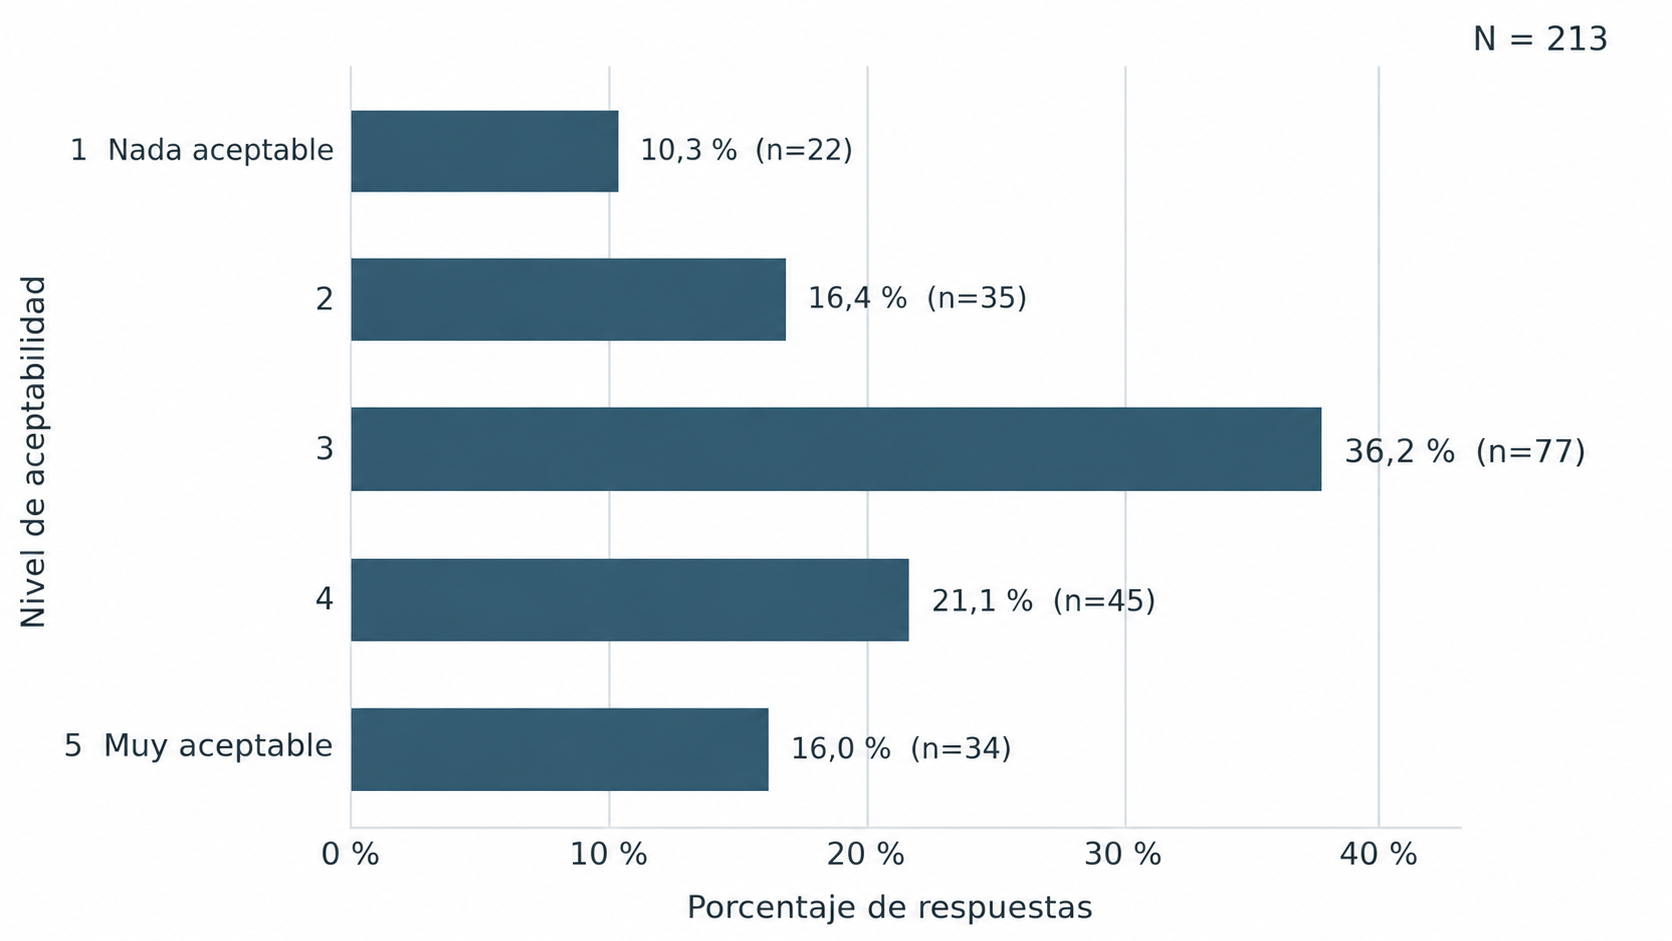
\includegraphics[width=0.85\textwidth]{./figures/ur_fig4_aceptabilidad}
    \caption[Aceptabilidad del registro de eventos de interacción]{Aceptabilidad del registro de eventos de interacción. Fuente: elaboración propia a partir de la encuesta de \textit{User Research}, $N=213$.}
    \label{fig:ur_aceptabilidad}
\end{figure}

La aceptabilidad del registro de eventos de interacción presentó una distribución heterogénea. El \textbf{37,1\,\%} manifestó niveles altos de aceptabilidad, mientras que el \textbf{36,2\,\%} se ubicó en el punto medio y el \textbf{26,8\,\%} seleccionó niveles bajos. Por lo tanto, los resultados no permiten asumir una aceptación generalizada de este tipo de registro, aun cuando la formulación presentada en la encuesta especificaba que no se almacenaría el contenido escrito. En consecuencia, la aceptabilidad del registro debe analizarse junto con las condiciones bajo las cuales se realiza la captura y el uso posterior de la información.

\begin{figure}[h!]
    \centering
    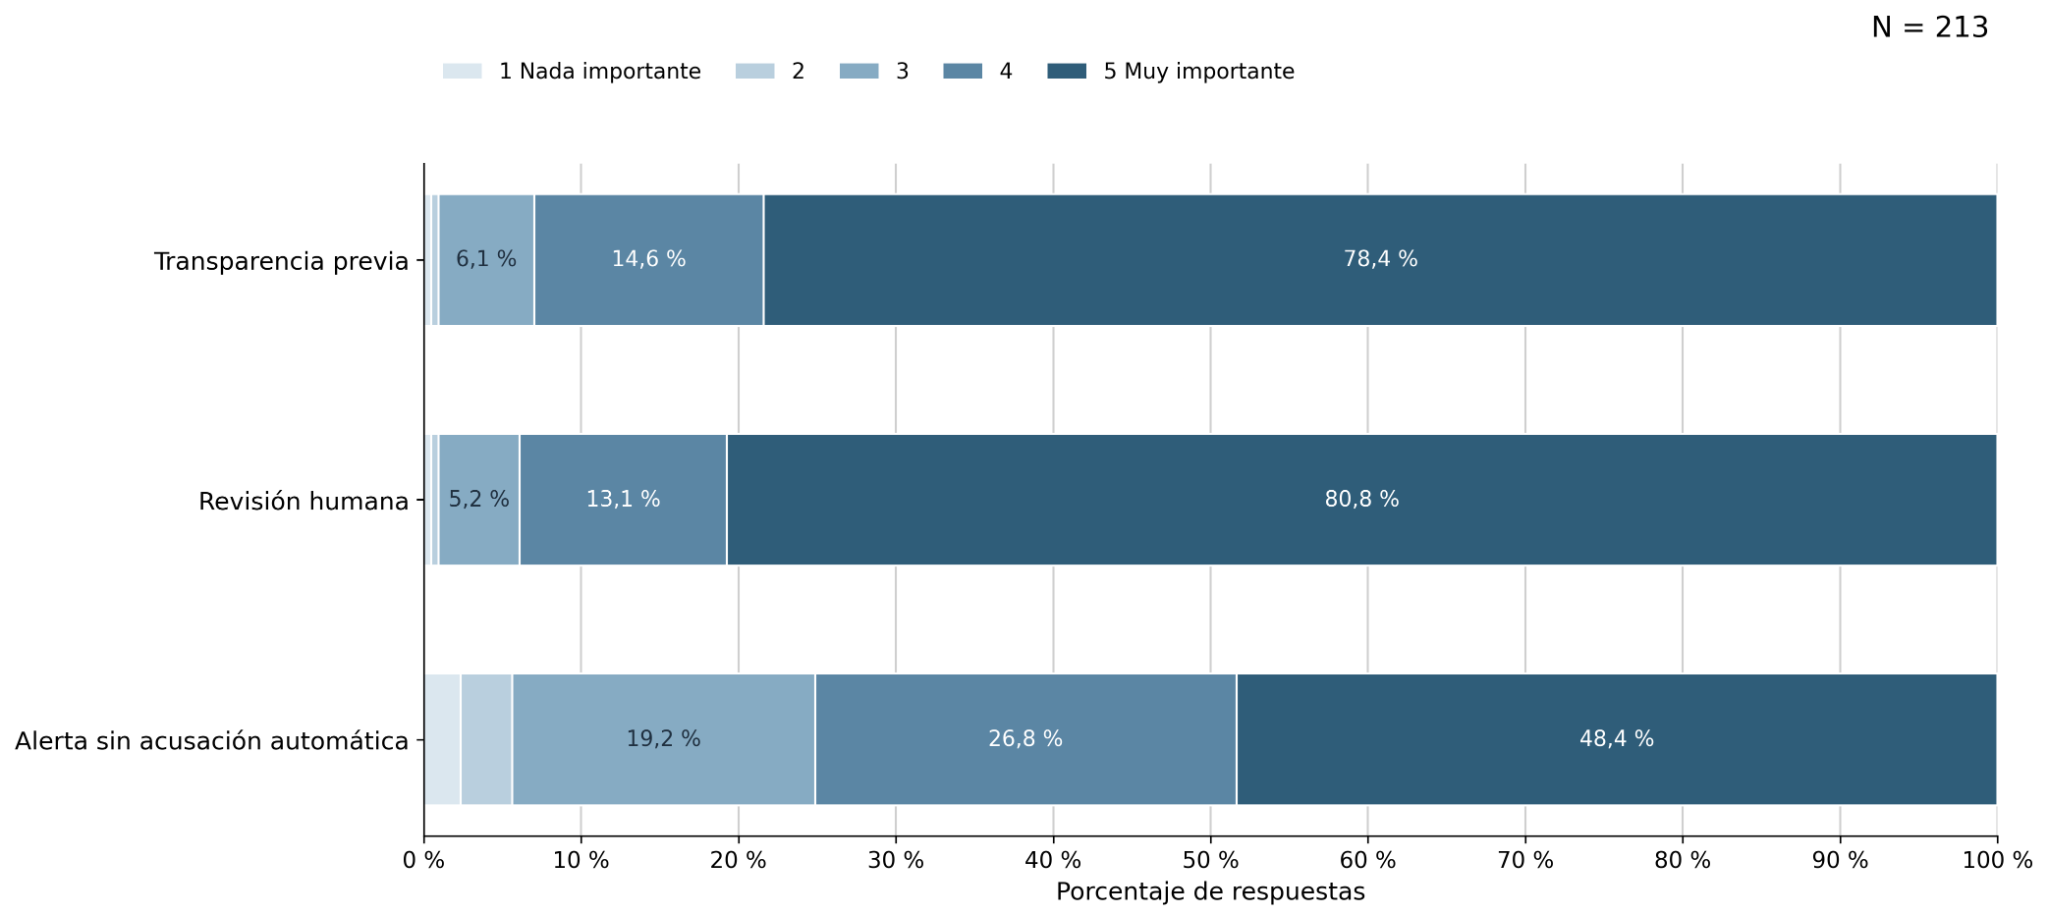
\includegraphics[width=0.85\textwidth]{./figures/ur_fig5_garantias}
    \caption[Importancia de las garantías asociadas a la supervisión]{Importancia de las garantías asociadas a la supervisión. Fuente: elaboración propia a partir de la encuesta de \textit{User Research}, $N=213$.}
    \label{fig:ur_garantias}
\end{figure}

Frente a las valoraciones más heterogéneas observadas sobre los mecanismos de supervisión, las condiciones vinculadas con su implementación presentan una tendencia considerablemente más definida. En la pregunta sobre transparencia previa (COM01), el \textbf{93,0\,\%} de la muestra asignó valores altos de importancia a conocer previamente qué datos se registran y con qué finalidad. En la pregunta sobre revisión humana (COM02), el \textbf{93,9\,\%} otorgó esa misma valoración a la existencia de revisión humana, mientras que en la pregunta sobre el límite a la acusación automática (EST15) el \textbf{75,1\,\%} consideró altamente importante que una alerta no implique de manera automática una acusación.

La pregunta sobre las acciones ante una situación atípica (EST14) complementa este resultado al distinguir entre la generación de una alerta y las acciones que pueden seguir a su detección. Ante una situación atípica, la opción individual más seleccionada fue generar una alerta para revisión humana posterior, con el \textbf{51,2\,\%} de las respuestas; un \textbf{20,7\,\%} eligió realizar una instancia adicional de validación y la anulación automática fue seleccionada por el \textbf{5,2\,\%}. Estas respuestas muestran una diferencia entre identificar un evento, revisarlo y determinar posteriormente qué acción corresponde, en lugar de tratar esas etapas como equivalentes.

En conjunto, los resultados muestran que las condiciones de implementación ---como la transparencia, la revisión humana y los límites a la automatización--- son aspectos especialmente valorados por la muestra y deben analizarse junto con el tipo de señal recolectada. La encuesta no determina por sí misma qué mecanismo de supervisión debería adoptarse. Estos resultados orientan a considerar, en etapas posteriores, la interpretabilidad de la información, el contexto de la evaluación y la existencia de instancias de revisión antes de derivar consecuencias académicas.

\section{Resultados cualitativos de las entrevistas}

El análisis de las entrevistas permitió profundizar en las condiciones que intervienen en la comprensión de la integridad académica en evaluaciones digitales. Las transcripciones completas de las entrevistas se incluyen en el Apéndice~\ref{apx:entrevistas}. Desde las perspectivas relevadas, una conducta no adquiere el mismo significado con independencia del contexto en el que ocurre: el tipo de evaluación, sus objetivos, el momento de la formación, los recursos autorizados y las reglas establecidas modifican la forma en que puede interpretarse una acción durante el examen. En su etapa de exploración, ENT-02 planteó que el uso y la interpretación de las herramientas deben ajustarse al momento de la formación profesional y al enfoque de cada evaluación.

La interpretación de las señales también apareció condicionada por la posibilidad de falsos positivos y por situaciones que admiten explicaciones legítimas. ENT-01 describió, a partir de su experiencia con mecanismos de supervisión ya implementados en UADE Online, casos en los que contingencias técnicas, notificaciones o movimientos del entorno podían ser registrados como incidencias sin que implicaran necesariamente una conducta indebida. ENT-02 relató una experiencia similar desde el lugar de estudiante frente a un sistema que generaba advertencias ante determinados comportamientos: ``Por ahí no estás haciendo nada raro e igual te pone un flag de advertencia.'' Además de la ambigüedad de la señal, ambos relatos incorporan una dimensión de fricción: determinados mecanismos pueden agregar presión al estudiante por la posibilidad de recibir advertencias o sufrir una interrupción de la evaluación aun cuando su comportamiento no responda a una intención de incumplir las reglas.

Esta posibilidad de error o ambigüedad otorga especial relevancia a la instancia de interpretación posterior. Al describir el funcionamiento de un sistema que realiza una clasificación preliminar de incidencias antes de que el docente revise los resultados, ENT-01 sostuvo: ``Yo siento que la curaduría humana del resultado tiene que estar siempre.'' En su experiencia, la revisión permite diferenciar incidencias relevantes de falsos positivos y considerar contingencias que un mecanismo automatizado puede registrar sin comprender su contexto.

La suficiencia de la evidencia constituyó otra dimensión relevante. Luego de la presentación del enfoque de ImprontIA, ENT-01 planteó específicamente la dificultad de utilizar determinados indicios cuando el estudiante puede cuestionar la evidencia que sustenta una decisión. La misma cuestión apareció de forma explícita en ENT-03, cuya participante planteó la necesidad de considerar para qué podría utilizarse la información obtenida y qué acciones podrían justificarse a partir de ella. Su observación introduce el problema de la accionabilidad: la utilidad de una señal no depende únicamente de que pueda ser capturada, sino también de qué interpretación puede realizarse y qué acciones resultan académicamente justificables a partir de ella.

En este marco, las validaciones complementarias aparecieron como una alternativa para abordar casos en los que la señal inicial no resultara suficiente. ENT-02 planteó que, según la extensión y gravedad de la situación detectada, podía recurrirse a una repregunta sobre una respuesta particular o a una instancia oral. En ese mismo tramo destacó la necesidad de que las reglas, las condiciones de aprobación y las consecuencias ante incumplimientos se encuentren definidas con anterioridad al examen.

Finalmente, las entrevistas mostraron que la revisión de señales introduce una dimensión operativa que no puede separarse de su utilidad. ENT-01 describió como desafío la formación de los docentes para interpretar reportes, adquirir autonomía en su revisión y distinguir casos relevantes de falsos positivos; ENT-02 señaló que el volumen de alertas condicionaría la posibilidad de realizar instancias adicionales de validación; y ENT-03 vinculó la utilidad de la información con los recursos necesarios para obtenerla y actuar sobre ella. En consecuencia, la carga de revisión y la escalabilidad emergen en este estudio como una consideración operativa relevante, aunque no cuantificada (Sección~\ref{sec:ur_limitaciones}): la generación de alertas supone también capacidad posterior para interpretarlas y gestionarlas.

\section{Triangulación y hallazgos}

La triangulación se realizó integrando los resultados de la encuesta a estudiantes con las perspectivas obtenidas mediante las entrevistas semiestructuradas (matriz completa en el Apéndice~\ref{apx:triangulacion}). La finalidad de esta instancia no fue tratar ambas fuentes como mediciones equivalentes, sino analizar de qué manera se relacionan evidencias producidas desde posiciones diferentes. A partir de esta integración se identificaron relaciones de convergencia cuando ambas fuentes aportaron evidencia compatible sobre una misma dimensión, de complementariedad cuando una permitió profundizar o contextualizar a la otra, y casos en los que un aspecto fue observado principalmente desde una de las técnicas.

\begin{table}[h!]
    \caption{Síntesis de hallazgos del \textit{User Research}}
    \label{tab:ur_hallazgos}
    \centering
    \small
    \begin{tabularx}{\textwidth}{p{4.6cm} X}
        \toprule
        \tblhead \textbf{Hallazgo} & \textbf{Implicación} \\
        \midrule
        La integridad en evaluaciones digitales es multidimensional y depende del contexto evaluativo. & Considerar evidencia múltiple y conservar el contexto académico en el que se produce cada señal, sin interpretar las situaciones relevadas como una medición de fraude real. \\
        \addlinespace[3pt]
        La ausencia de cámara no implica por sí misma una menor percepción de invasividad. & Priorizar proporcionalidad, minimización de datos y transparencia; no afirmar que ImprontIA sea, sin más, menos invasivo que otras soluciones. \\
        \addlinespace[3pt]
        Transparencia, revisión humana y límites a la automatización son condiciones centrales del procedimiento. & Mantener diferenciadas la generación de señales y la adopción automática de una decisión académica. \\
        \addlinespace[3pt]
        Una alerta y una decisión académica constituyen etapas distintas. & Tratar una alerta como información preliminar capaz de orientar una revisión o validación, y no como un veredicto. \\
        \addlinespace[3pt]
        Los falsos positivos y la ambigüedad limitan la interpretación aislada de una señal. & Presentar las señales junto con su contexto y admitir explicaciones alternativas antes de inferir su significado académico. \\
        \addlinespace[3pt]
        Las validaciones complementarias permiten profundizar casos de evidencia incierta. & Utilizar una señal incierta para orientar una profundización selectiva de la evaluación, sin inferir que toda alerta requiera una nueva instancia. \\
        \bottomrule
    \end{tabularx}
\end{table}

La integración de las fuentes muestra, en primer lugar, que el problema no puede reducirse a la detección de una conducta aislada. Al mismo tiempo, aumentar la supervisión no elimina necesariamente las tensiones: los mecanismos utilizados pueden introducir problemas de invasividad, fricción o ambigüedad. En este marco, las condiciones procedimentales adquieren una relevancia transversal, particularmente la transparencia, la revisión humana y la separación entre la detección de un evento y una consecuencia académica.

Los hallazgos también ponen en primer plano la relación entre la fuerza de la evidencia y la decisión que se pretende adoptar. Una señal puede ser suficiente para orientar una revisión o una comprobación adicional sin serlo para sostener una acusación o invalidación. La proporcionalidad, por lo tanto, no se refiere únicamente al mecanismo de supervisión utilizado, sino también a la relación entre la información disponible y la acción posterior que se pretende justificar.

Finalmente, la carga docente y la escalabilidad ---ya señaladas como consideración exploratoria--- se mantienen fuera de los seis hallazgos centrales de la Tabla~\ref{tab:ur_hallazgos}, dado que las entrevistas no permiten cuantificarlas.

\begin{keyfinding}{Los tres hallazgos con mayor impacto directo sobre el diseño}
\begin{enumerate}
    \item La ausencia de cámara \textbf{no} implica por sí misma una menor percepción de invasividad, lo que relativiza un supuesto inicial del proyecto.
    \item Transparencia previa (\textbf{93,0\,\%}) y revisión humana (\textbf{93,9\,\%}) son, con amplio margen, las condiciones más valoradas por la muestra.
    \item Una alerta y una decisión académica son etapas distintas para los participantes: solo el \textbf{5,2\,\%} seleccionó la anulación automática como acción ante una situación atípica.
\end{enumerate}
\end{keyfinding}

\section{Perfiles de usuario}

A partir de los resultados presentados en las secciones anteriores se construyeron tres perfiles de usuario (\textit{personas}) que sintetizan actitudes, necesidades, objetivos y frustraciones relevadas: Santiago, estudiante, y Laura, docente universitaria, que corresponden a los dos actores funcionales definidos en el Capítulo~\ref{ch:requerimientos}, y Marcela, coordinadora de educación a distancia, que representa a la institución que decide adoptar y gestionar una herramienta de supervisión. Las frases síntesis atribuidas a cada perfil fueron construidas a partir de los hallazgos del estudio, describen necesidades y tensiones del problema, no características de una solución, y no son citas textuales de un participante individual.

El respaldo empírico de los perfiles es desigual. Santiago se apoya en la encuesta a estudiantes y en los relatos de experiencia como estudiante de las entrevistas; Laura y Marcela se apoyan solo en las tres entrevistas, por lo que deben leerse como hipótesis de trabajo a validar con una muestra docente e institucional más amplia (Sección~\ref{sec:ur_limitaciones}).

Santiago sintetiza al actor Estudiante: su tensión central es rendir bajo reglas claras y previsibles, sabiendo de antemano qué se observa durante la evaluación y con la posibilidad de explicar situaciones que puedan parecer irregulares sin serlo. Laura sintetiza al actor Docente/Evaluador: su tensión central es distinguir, con el tiempo de revisión disponible, qué situaciones merecen su atención y contar con elementos para fundamentar su criterio académico. Marcela sintetiza la perspectiva institucional: su tensión central es sostener evaluaciones digitales confiables a escala, con docentes capacitados para interpretar lo que se registra y con decisiones que puedan justificarse ante un reclamo.

\begin{table}[h!]
    \caption{Síntesis de los perfiles de usuario}
    \label{tab:personas_resumen}
    \centering
    \small
    \begin{tabularx}{\textwidth}{p{2.3cm} p{3.4cm} X}
        \toprule
        \tblhead \textbf{Persona} & \textbf{Rol} & \textbf{Necesidad central} \\
        \midrule
        \textbf{Santiago} & Estudiante de Sistemas & Rendir con reglas claras y previsibles y saber de antemano qué se observa durante la evaluación. \\
        \textbf{Laura} & Docente universitaria & Distinguir qué situaciones merecen su atención y fundamentar su criterio académico con el tiempo disponible. \\
        \textbf{Marcela} & Coordinadora de educación a distancia & Sostener evaluaciones confiables a escala, con docentes capacitados y decisiones justificables ante un reclamo. \\
        \bottomrule
    \end{tabularx}
\end{table}

El detalle completo de los tres perfiles ---actitudes y criterios, necesidades, objetivos y frustraciones, tal como fueron diseñados a partir de este estudio--- se presenta en el Apéndice~\ref{apx:personas}.

\section{Síntesis de aprendizaje}

El \textit{User Research} permitió precisar el planteo inicial del problema a partir de las percepciones estudiantiles y de las perspectivas relevadas en docencia, investigación y gestión académica. Los resultados respaldan la existencia de una cuestión relevante vinculada con la confianza y la integridad en las evaluaciones digitales, pero muestran que no puede caracterizarse a partir de una única conducta o mecanismo de control. Los riesgos percibidos son diversos y su interpretación depende de las características de cada instancia evaluativa, sus objetivos, las reglas establecidas y los recursos permitidos.

Uno de los principales aprendizajes fue relativizar el supuesto de que la ausencia de cámara implica necesariamente una menor percepción de invasividad. Los resultados de la encuesta no permiten sostener esa relación de manera general, del mismo modo que la evidencia relevada tampoco permite asumir que una mayor observación produzca necesariamente mayor confianza, que un mayor volumen de alertas implique mayor utilidad o que una anomalía constituya por sí sola evidencia suficiente de deshonestidad.

En este proceso adquirieron mayor relevancia dimensiones vinculadas con la transparencia, la proporcionalidad, la revisión humana, la ambigüedad de las señales, la posibilidad de actuar sobre la información obtenida, la definición previa de reglas y el contexto de cada evaluación. A estas dimensiones se agrega una consideración operativa: la información generada solo puede resultar útil en la medida en que pueda ser interpretada y gestionada dentro de una carga de revisión razonable. Estos aprendizajes precisan el problema investigado, de acuerdo con el alcance definido para esta etapa.

\section{Formulación del problema luego del \textit{User Research}}

A partir de los resultados obtenidos, se reformuló el planteo inicial incorporando la multiplicidad de situaciones relevadas, la dependencia del contexto evaluativo y las condiciones necesarias para interpretar de manera prudente la evidencia producida durante una evaluación digital.

En las evaluaciones digitales, sostener condiciones de integridad y confianza resulta complejo porque el proceso de resolución ofrece señales que pueden ser múltiples, contextuales y ambiguas. Los mecanismos de supervisión pueden aportar evidencia, pero también introducen tensiones de privacidad, invasividad y falsos positivos; a su vez, las alertas requieren interpretación, reglas transparentes y revisión humana para que puedan utilizarse de manera proporcional y académicamente defendible.

\section{Limitaciones}
\label{sec:ur_limitaciones}

Los resultados deben interpretarse dentro del alcance del estudio realizado. La encuesta se aplicó sobre una muestra estudiantil no probabilística por conveniencia y, por lo tanto, sus resultados no son generalizables a la totalidad de la población universitaria. Además, existe un predominio de participantes pertenecientes a Ingeniería, Tecnología e Informática, y el estudio no reporta un desglose por institución. El tamaño de la muestra ($N=213$) permite describir sus percepciones con cierta estabilidad, pero no asegura que sea representativa del público objetivo de los perfiles: no se cuantificó qué proporción de los participantes coincide con el perfil de Santiago (estudiante de carreras de sistemas con experiencia en evaluaciones digitales), y los perfiles de Laura y Marcela no cuentan con respaldo de encuesta, sino solo de las entrevistas. La información obtenida corresponde a percepciones autoinformadas y no a observaciones directas del comportamiento durante evaluaciones; en consecuencia, el estudio no midió objetivamente la ocurrencia de fraude, la frecuencia de falsos positivos ni el impacto de los mecanismos de supervisión sobre el desempeño académico.

El componente cualitativo estuvo compuesto por tres entrevistas semiestructuradas vinculadas con perspectivas de docencia, investigación y gestión académica, sin incluir entrevistas individuales con estudiantes. Una de ellas se realizó con un docente con quien los entrevistadores tenían un vínculo previo docente--alumno, posible fuente de sesgo de complacencia. Además, ENT-01 dirige UADE Online y ENT-03 se desempeña en el Departamento de Educación a Distancia de esa misma área; es decir, ambos trabajan en la institución en la que estudian los autores y con los mecanismos de supervisión de evaluaciones que UADE utiliza hoy. Este vínculo institucional se declara como posible fuente de sesgo en dos direcciones: una tendencia a defender o justificar los mecanismos vigentes, de los que son responsables, y una disposición favorable hacia un proyecto de estudiantes de la propia universidad. Para acotarlo, en ENT-01 la exploración del problema se realizó antes de presentar ImprontIA, los aportes de ENT-03 se trataron como retroalimentación y no como hallazgos espontáneos, y ninguna conclusión del capítulo se apoya solo en estas entrevistas: todas se contrastaron con la encuesta en la matriz de triangulación (Apéndice~\ref{apx:triangulacion}). Parte de las observaciones se obtuvo después de presentar el enfoque general de ImprontIA y se analizó como retroalimentación posterior, diferenciándola de la etapa de exploración. En particular, ENT-03 no cuenta con un tramo de \textit{discovery} limpio directamente comparable con los de ENT-01 y ENT-02. Por último, si bien la carga docente y la escalabilidad surgieron como consideraciones relevantes en las entrevistas, el estudio no cuantificó tiempos, costos ni volúmenes de revisión asociados.

\section{Implicaciones para las siguientes etapas}

Los resultados del \textit{User Research} establecen orientaciones para las etapas posteriores del proyecto sin definir todavía características funcionales o técnicas de la propuesta. En primer lugar, sugieren considerar evidencia múltiple y conservar el contexto en el que se produce cada señal, favoreciendo información que pueda ser interpretada en relación con el tipo, los objetivos y las reglas de la evaluación. Asimismo, la captura de información deberá analizarse desde criterios de minimización y proporcionalidad, junto con una comunicación transparente acerca de qué se registra y con qué finalidad.

La diferenciación observada entre una alerta, su revisión y una eventual consecuencia académica orienta a mantener estas instancias separadas. Las señales atípicas pueden aportar información para una revisión posterior o para una validación complementaria en situaciones ambiguas, pero no deberían interpretarse por sí mismas como acusaciones o sanciones automáticas.

Finalmente, la utilidad de la información generada debe analizarse también desde su viabilidad operativa. Un mayor volumen de señales no implica necesariamente una mayor capacidad de decisión si la información producida resulta difícil de interpretar o genera una carga de revisión que no puede ser gestionada. Estas orientaciones sirvieron como insumo directo para el análisis de requerimientos (Capítulo~\ref{ch:requerimientos}) y para el análisis competitivo (Sección~\ref{ch:competencias}).

Los apéndices asociados a este capítulo reproducen los perfiles de usuario completos (Apéndice~\ref{apx:personas}), el instrumento de encuesta aplicado (Apéndice~\ref{apx:encuesta}), las transcripciones íntegras de las entrevistas (Apéndice~\ref{apx:entrevistas}), el \textit{codebook} y la matriz temática del análisis cualitativo (Apéndice~\ref{apx:cualitativo}) y la matriz de triangulación completa (Apéndice~\ref{apx:triangulacion}).
